\chapter{Studi Literatur}

Bab ini akan berisi pembahasan dari studi literatur yang akan berkaitan dengan permasalahan yang dibahas di Tugas Akhir ini. Hasil studi literatur akan menjadi dasar dalam pengerjaan Tugas Akhir ini baik untuk menganalisis masalah dan juga untuk merancang solusi.

\section{Distributed Tracing}
\label{bab2-dtracing}

\subsection{\textit{Overview} Distributed Tracing}
Dengan meningkatnya penggunaan Microservice, cara untuk melakukan \textit{profiling}, \textit{debugging}, dan \textit{monitoring} aplikasi menjadi berbeda dengan cara yang dilakukan pada aplikasi yang berbentuk Monolith.
Salah satu cara untuk melakukan profiling pada aplikasi berbasis Microservice adalah dengan Distributed Tracing.
Distributed Tracing, disebut juga dengan Distributed Request Tracing, adalah sebuah tipe logging terkorelasi yang dapat memberikan pengguna mendapatkan visibilitas pada operasi dari perangkat lunak terdistribusi untuk kasus seperti debugging di environment \textit{production}, dan analisis penggalian akar masalah pada kegagalan atau insiden lainnya \citep{parker2020distributed}.
Dengan adanya kakas Distributed Tracing, pengguna dapat mendapatkan insight mengenai operasi yang terjadi di aplikasi terdistribusi secara kolektif dengan cara melakukan pelacakan pada \textit{request} yang dibuat oleh suatu \textit{service}.

Kita bisa sebut setiap pekerjaan yang dilakukan oleh sebuah \textit{service} dalam suatu waktu sebagai \textit{span}.
Setiap \textit{span} bisa diisi dengan \textit{metadata}, seringkali disebut sebagai \textit{attributes} atau \textit{tags}, dan \textit{events}, seringkali disebut sebagai \textit{logs}.
Setiap pemanggilan Remote Procedure Call (RPC) atau Application Programming Interface (API) antara \textit{service} akan merepresentasikan hubungan dari \textit{request} yang terjadi diantara \textit{service} tersebut.
Hubungan tersebut disebarkan diantara \textit{service} sebagai \textit{trace context}, yaitu data yang secara unik mendefinisikan \textit{span} yang dibuat oleh setiap \textit{service}.
Setiap \textit{span} yang dibuat oleh setiap \textit{service} tersebut diteruskan kepada proses eksternal yang dapat dikumpulkan atau diagregasi sebagai sebuah \textit{trace}.
\textit{Trace} tersebut dapat dianalisis lebih lanjut dan disimpan untuk mendapatkan \textit{insight} mengenai \textit{service}.
Berikut adalah ilustrasi sederhana mengenai \textit{trace}:
\begin{figure}[htb]
      \centering
      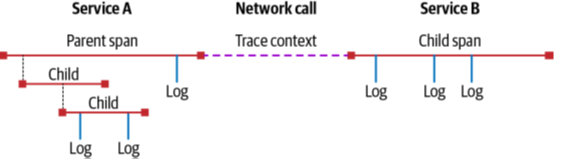
\includegraphics[width=1\textwidth]{resources/ch2/tracing-illus.png}
      \caption{Ilustrasi \textit{Tracing} \citep{parker2020distributed}}
      \label{ch2-trace-illus}
\end{figure}

Salah satu keuntungan dari penggunaan \textit{distributed tracing} adalah \textit{span} yang dihasilkan akan terisolasi dan independen satu sama lain. Sehingga suatu \textit{span} tertentu hanya menggambarkan aliran \textit{request} yang dapat mencakup keseluruhan aplikasi. Gambar \ref{ch2-span} menggambarkan sebuah \textit{span} yang memiliki "anak" \textit{span} yang tergabung dalam sebuah "induk" \textit{span} sehingga suatu \textit{span} dapat menggambarkan konteks suatu \textit{request} yang terjadi tidak hanya pada satu \textit{service} saja, namun juga mencakup operasi yang ada di dalamnya dan jika \textit{request} mencakup aksi \textit{service} lainnya akan tercatat "anak" dari \textit{span} tersebut.
\begin{figure}[htb]
	\centering
	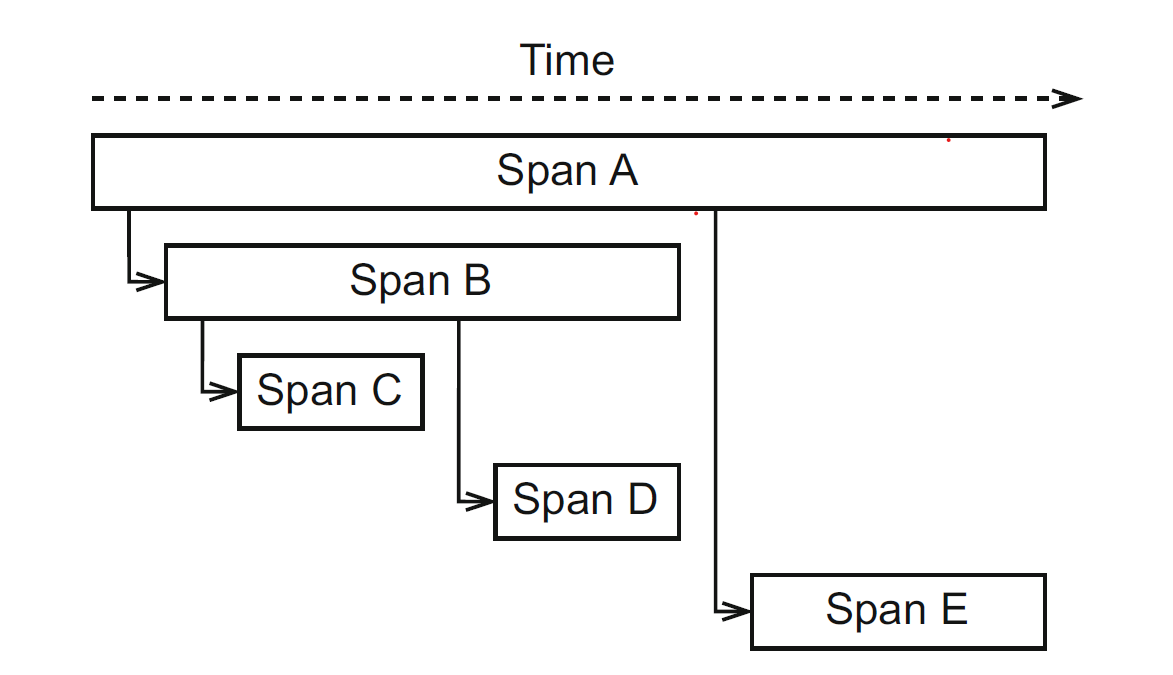
\includegraphics[width=0.8\textwidth]{resources/ch2/trace-ilus-2.png}
	\caption{Ilustrasi \textit{Span} sepanjang waktu \citep{bento2021}}
	\label{ch2-span}
\end{figure}


Adapun komponen-komponen yang membangun sistem Distributed Tracing adalah sebagai berikut \citep{parker2020distributed}:
\begin{enumerate}
      \item Instrumentasi \\
            Distributed Tracing membutuhkan data \textit{trace} agar dapat bekerja.
            Data \textit{trace} dihasilkan dengan cara menginstrumentasikan proses-proses \textit{service} atau mentrasformasikan data telemetri yang sudah ada ke data \textit{trace}.
      \item \textit{Deployment} \\
            Setelah data \textit{trace} dihasilkan, kita perlu mengirimkan data tersebut ke suatu tempat.
            Melakukan \textit{deployment} pada sistem \textit{tracing} membutuhkan pemahaman dimana perangkat lunak kita dijalankan di \textit{server} dan bagaimana perangkat tersebut dijalankan.
            Agar dapat memaksimalkan kemampuan dari \textit{tracing} juga meminimalkan \textit{overhead} yang terjadi pada aplikasi, kita perlu memahami teknik yang cocok untuk melakukan deployment pada sistem Distributed Tracing yang akan kita gunakan.
      \item Penyampaian \textit{Value} \\
            Saat \textit{service} kita telah dapat menghasilkan data \textit{trace} dan kita telah memiliki infrastruktur yang diperlukan untuk mengolah data \textit{trace} tersebut, kita akan memerlukan kakas yang tepat untuk menggabungkan \textit{trace} dari berbagai \textit{service} dengan metadata lain seperti \textit{metrics} dan \textit{logs} untuk dapat menghasilkan \textit{value} yang berguna bagi proses \textit{debugging}, \textit{profiling}, dan \textit{monitoring} perangkat lunak terdistribusi.
\end{enumerate}

%\subsection{\textit{Context Propagation}}

\subsection{Mendefinisikan \textit{Critical Path}}
\label{crit-path}

%\subsection{Komponen Distributed Tracing}
%
%\subsubsection{Instrumentasi}
%
%\subsubsection{\textit{Deployment}}
%
%\subsubsection{\textit{Value Delivery}}

%\subsection{Pelacakan \textit{request causality}}
%\label{bab2-dtracing-causality}
\section{HTTP/2}

\section{gRPC}
gRPC adalah sebuah \textit{framework} Remote Procedure Call (RPC) Open Source berperforma tinggi yang dapat dijalankan di berbagai environment \citep{grpc}.
gRPC dapat secara efisien menghubungkan \textit{service} yang berada di dalam dan antara data center dengan berbagai dukungan untuk melakukan load balancing, tracing, pengecekan kesehatan, dan autentikasi.
gRPC juga dapat diaplikasikan pada server yang terdistribusi untuk menghubungkan berbagai perangkat mulai dari aplikasi mobile dan browser ke layanan backend.
Seperti RPC pada umumnya, gRPC memungkinkan \textit{service} yang terpisah untuk mengakses fungsi layaknya objek lokal. Ada beberapa skenario penggunaan utama dari gRPC:
\begin{enumerate}
	\item Menghubungkan service-service yang bersifat poliglot seperti dalam arsitektur Microservice.
	\item Menghubungkan perangkat mobile, browser client ke service backend.
	\item Menghasilkan library bagi sisi client yang efisien.
\end{enumerate}

Secara default, gRPC menggunakan Protocol Buffers sebagai Interface Definition Language (IDL) dan juga sebagai format pertukaran pesannya (walaupun juga bisa menggunakan JSON sebagai format pertukaran data).
Langkah pertama ketika menggunakan Protocol Buffers adalah dengan mendefinisikan struktur dari data yang ingin diserialisasi dalam sebuah file proto, yaitu sebuah file teks biasa yang memiliki ekstensi “.proto”.
Data dari Protocol Buffers distrukturkan sebagai messages yang masing-masing memiliki catatan mengenai data yang berbentuk pasangan name-value yang disebut dengan fields.
Berikut adalah contoh sederhana dari file proto:
\lstinputlisting[captionpos=b, caption={Contoh File Proto}]{codes/ch2/hello.proto}

Ketika struktur data sudah dibuat, kode Proto tersebut perlu di compile menggunakan kakas bernama protoc yang akan membuat akses data dalam bahsa pemrograman yang dipilih.
gRPC menggunakan protoc untuk menghasilkan kode dari file Proto berupa: kode gRPC bagi client dan server, dan juga kode Protocol Buffer biasa yang digunakan untuk melakukan populasi, serialisasi, dan kode untuk mendapatkan tipe pesan.

Adapun penggunaan gRPC pada sistem client dan server adalah sebagai berikut:
\begin{enumerate}
	\item Mendefinisikan service beserta method apa saja yang bisa dipanggil beserta parameter dan juga return type bagi masing-masing method.
	\item  Server akan mengimplementasi interface hasil kompilasi protoc yang berasal dari method-method yang didefinisikan pada file proto.
	\item Client akan memanggil method yang sudah didefinisikan pada server.
\end{enumerate}



%\section{Protokol Komunikasi Microservice}
%Pada subbab ini akan dijelaskan beberapa protokol komunikasi yang bisa digunakan dalam arsitektur Microsevice.
%\subsection{REST API}
%Representational State Transfer (REST) merupakan sebuah gaya arsitektur yang dibuat untuk mendesain sistem yang berjalan di World Wide Web.
%REST pertama kali diperkenalkan oleh Roy Thomas Fielding dalam disertasinya pada tahun 2005 yang berjudul \textit{Architectural Styles and the Design of Network-based Software Architectures}.
%Dalam mendesain arsitektur, REST mendefinisikan beberapa aturan yaitu skalabilitas antara komponen yang berinteraksi, antar muka yang seragam, \textit{deployment} yang independen bagi komponen, dan pembuatan arsitektur berlapis yang dapat memfasilitasi komponen untuk melakukan \textit{caching} agar dapat mengurangi \textit{latency}, memperkuat \textit{security}, dan mengenkapsulasi sistem \textit{legacy} \citep{rest}.
%
%Application Programming Interface (API) yang didesain berdasarkan prinsip-prinsip REST disebut dengan RESTful API.
%Ada dua konsep utama yang dipakai dalam mendesain REST API yaitu \textit{resources}, atau sumber daya, dan \textit{representations}, atau representasi \citep{restful-book}.
%Resource yang dimaksud dalam konteks RESTful API bisa berarti apa saja yang cukup penting untuk direferensi dan diakses sebagai API.
%Sebuah \textit{resource} biasanya sesuatu yang dapat disimpan dalam komputer seperti sebuah data yang disimpan dalam database ataupun sebuah hasil dari eksekusi algoritme.
%Satu-satunya batasan pada setiap \textit{resource} tersebut adalah setiap resource harus memiliki sebuah URL.
%Representasi sendiri menggambarkan bagaimana kondisi atau \textit{\textit{state}} saat \textit{resource} tersebut diakses.
%Contoh paling umum dari representasi  RESTful API adalah mentransportasikan \textit{resource} melalui protokol HTTP dan dalam bentuk data JSON.
%
%Dalam praktiknya, \textit{resource} sendiri tidak bisa diakses dengan sembarang cara.
%Dalam sistem RESTful API, client dan server berinteraksi dengan saling mengirim pesan yang mengikuti protokol yang sudah ditentukan sebelumnya, dalam hal ini adalah mengikuti semantik dari protokol HTTP itu sendiri.
%HTTP mendefinisikan delapan jenis pesan yang berbeda, namun ada empat yang paling sering digunakan, yaitu:
%\begin{enumerate}
%      \item GET \\
%            Dapatkan representasi dari sebuah \textit{resource}.
%      \item DELETE \\
%            Hapus \textit{resource} tersebut.
%      \item POST \\
%            Buat sebuah \textit{resource} berdasarkan representasi yang diberikan.
%      \item PUT \\
%            Gantikan \textit{state} dari \textit{resource} yang dimaksud sesuai dengan representasi yang diberikan.
%\end{enumerate}
%
%Dalam penggunaannya bagi komunikasi Microservice, RESTful API melalui HTTP masih menjadi pilihan yang paling banyak digunakan oleh developer menurut survey yang dilakukan oleh The Software House pada tahun 2020 \citep{tsh2020}.
%Walaupun adopsi nya sebagai protokol komunikasi Microservice cukup populer, namun ada beberapa kekurangan dari RESTful API \citep{web-service-article} yaitu:
%\begin{enumerate}
%      \item Tidak cocok untuk data dalam jumlah besar
%      \item Latency dan Overhead dalam pemrosesan request karena pengunaan protokol HTTP
%      \item	RESTful API memiliki ketergantungan tinggi pada Header untuk mengatur \textit{state}
%\end{enumerate}
%
%\subsection{GraphQL}
%GraphQL merupakan sebuah bahasa query dan manipulasi untuk API dan runtime untuk memenuhi query tersebut dengan data yang sudah ada \citep{graphql}.
%GraphQL dikembangkan oleh Facebook sebelum dirilis ke publik sebagai proyek Open Source pada tahun 2015.
%Pendekatan GraphQL dalam membuat API seringkali dikontraskan dengan metode pembuatan API yang sudah ada seperti REST.
%Perbedaan utama antara pendekatan GraphQL adalah cara menstrukturkan data yang diekspos ke API.
%REST melakukan penstrukturan data berdasarkan \textit{resource} sementara GraphQL menstrukturkan data lewat query yang dispesifikkan oleh pengguna seperti SQL.
%
%Sebuah layanan GraphQL dibuat dengan cara mendefinisikan tipe-tipe data pada masing-masing \textit{field}-nya kemudian menyediakan masing-masing fungsi untuk setiap \textit{field} pada tipe data tersebut.
%
%\lstinputlisting[captionpos=b, caption={Definisi Query Data}]{codes/ch2/example.graphql}
%
%\lstinputlisting[captionpos=b, caption={Fungsi Handler}]{codes/ch2/graphql-handler.js}
%
%Dari tipe data yang didefinisikan di atas, berikut adalah contoh query GraphQL beserta response-nya:
%
%\lstinputlisting[captionpos=b, caption={Query GraphQL}]{codes/ch2/query.graphql}
%
%\lstinputlisting[captionpos=b, caption={\textit{Response} GraphQL dalam JSON}]{codes/ch2/response.json}
%
%\subsection{gRPC}
%gRPC adalah sebuah \textit{framework} Remote Procedure Call (RPC) Open Source berperforma tinggi yang dapat dijalankan di berbagai environment \citep{grpc}.
%gRPC dapat secara efisien menghubungkan \textit{service} yang berada di dalam dan antara data center dengan berbagai dukungan untuk melakukan load balancing, tracing, pengecekan kesehatan, dan autentikasi.
%gRPC juga dapat diaplikasikan pada server yang terdistribusi untuk menghubungkan berbagai perangkat mulai dari aplikasi mobile dan browser ke layanan backend.
%Seperti RPC pada umumnya, gRPC memungkinkan \textit{service} yang terpisah untuk mengakses fungsi layaknya objek lokal. Ada beberapa skenario penggunaan utama dari gRPC:
%\begin{enumerate}
%      \item Menghubungkan service-service yang bersifat poliglot seperti dalam arsitektur Microservice.
%      \item Menghubungkan perangkat mobile, browser client ke service backend.
%      \item Menghasilkan library bagi sisi client yang efisien.
%\end{enumerate}
%
%Secara default, gRPC menggunakan Protocol Buffers sebagai Interface Definition Language (IDL) dan juga sebagai format pertukaran pesannya (walaupun juga bisa menggunakan JSON sebagai format pertukaran data).
%Langkah pertama ketika menggunakan Protocol Buffers adalah dengan mendefinisikan struktur dari data yang ingin diserialisasi dalam sebuah file proto, yaitu sebuah file teks biasa yang memiliki ekstensi “.proto”.
%Data dari Protocol Buffers distrukturkan sebagai messages yang masing-masing memiliki catatan mengenai data yang berbentuk pasangan name-value yang disebut dengan fields.
%Berikut adalah contoh sederhana dari file proto:
%\lstinputlisting[captionpos=b, caption={Contoh File Proto}]{codes/ch2/hello.proto}
%
%Ketika struktur data sudah dibuat, kode Proto tersebut perlu di compile menggunakan kakas bernama protoc yang akan membuat akses data dalam bahsa pemrograman yang dipilih.
%gRPC menggunakan protoc untuk menghasilkan kode dari file Proto berupa: kode gRPC bagi client dan server, dan juga kode Protocol Buffer biasa yang digunakan untuk melakukan populasi, serialisasi, dan kode untuk mendapatkan tipe pesan.
%
%Adapun penggunaan gRPC pada sistem client dan server adalah sebagai berikut:
%\begin{enumerate}
%      \item Mendefinisikan service beserta method apa saja yang bisa dipanggil beserta parameter dan juga return type bagi masing-masing method.
%      \item  Server akan mengimplementasi interface hasil kompilasi protoc yang berasal dari method-method yang didefinisikan pada file proto.
%      \item Client akan memanggil method yang sudah didefinisikan pada server.
%\end{enumerate}
%
%\subsection{WebSocket}



%\section{\textit{Observability} pada Sistem Terdistribusi}
%\label{bab2-observability}

\section{Kubernetes}
\subsection{Arsitektur Kubernetes}
Arsitektur Kubernetes terdiri atas dua macam node yaitu master node dan worker node.
Setiap cluster Kubernetes terdiri dari minimal satu buah worker node dan satu atau lebih worker node.
Master node akan mengatur semua worker node dan pod yang ada di dalam cluster.
Dalam environment production, biasanya master node akan berjalan di beberapa komputer dan cluster akan berjalan dengan beberapa node sehingga menyediakan sifat fault-tolerance dan high-availability \citep{kube-arch}.
Untuk mengakses cluster Kubernetes, pengguna akan menspesifikkan perintah kepada master node melalui aplikasi command line bernama kubectl dan master node akan menyesuaikan state yang diminta oleh pengguna dengan memberikan perintah kepada worker node yang tersedia seperti membuat pod baru.
Berikut adalah gambaran arsitektur Kubernetes:
\begin{figure}[htb]
      \centering
      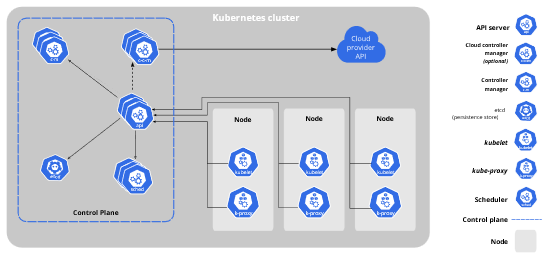
\includegraphics[width=0.9\textwidth]{resources/ch2/kube-1.png}
      \caption{Arsitektur Kubernetes \citep{kube-arch}}
      \label{KubeArch}
\end{figure}

Adapun komponen-komponen yang terdapat pada master node antara lain:
\begin{enumerate}
      \item Kube-apiserver adalah komponen dari master node yang mengekspos API Kubernetes. API Server adalah frontend dari worker node / control plane bagi Kubernetes.
      \item Etcd adalah komponen yang berfungsi sebagai penyimpan data yang konsisten dan higly-available dengan skema penyimpanan key-value.
      \item	Kube-scheduler berfungsi sebagai pengawas dan penjadwal bagi pod yang baru dibuat dan tugasnya adalah untuk menetapkan dimana node  bagi pod tersebut.
      \item	Kube-controller-manager adalah komponen yang berfungsi untuk menjalankan proses controller yaitu fungsi yang bertanggung jawab mengelola pod, worker node, dan mengatur tugas jika terjadi kegagalan pada proses pembuatan pod.
\end{enumerate}

Adapun komponen-komponen yang terdapat pada worker node antara lain:
\begin{enumerate}
      \item  Kubelet adalah komponen yang berfungsi sebagai agen di setiap node yang ada pada cluster dan bertugas untuk memastikan container yang berjalan pada pod.
      \item Kube-proxy adalah sebuah proxy jaringan yang berjalan di setiap node pada cluster dan mengimplementasikan konsep dari service Kubernetes.
      \item Container Runtime adalah sebuah perangkat lunak yang bertanggung jawab untuk menjalankan container. Kubernetes sendiri mendukung beberapa Container Runtime seperti Docker, containerd, CRI-O, dan semua jenis Runtime yang mengimplementasi Kubernetes CRI (Container Runtime Interface).
\end{enumerate}

\subsection{Pod}
Pod adalah unit terkecil yang dapat di deploy di dalam sebuah Kubernetes cluster.
Pod sendiri adalah sebuah abstraksi dari container yang di deploy di Kubernetes.
Jadi, ketika seorang pengguna ingin membuat sebuah aplikasi berbasis container di Kubernetes, pengguna tidak melakukan deploy container secara langsung melainkan melalui object Kubernetes yang bernama Pod.
Di dalam Pod sendiri bisa terdapat lebih dari satu buah container sekaligus sesuai dengan kebutuhan.
Contohnya ada jenis container yang disebut sebagai sidecar yang berfungsi sebagai secondary unit dari container utama yang ada di dalam Pod tersebut.
\subsection{Controller}
Kita bisa langsung membuat Pod di kubernetes lewat command line interface.
Namun jika kita membuat secara manual Pod, maka kita juga harus bertanggung jawab selama lifecycle dari Pod tersebut.
Masalah timbul ketika kita ingin membuat beberapa Pod yang sama sekaligus, maka akan menjadi suatu tugas yang tidak mudah untuk mengatur Pod-Pod tersebut.
Dari permasalahan itulah, ada sebuah konsep di Kubernetes yang disebut dengan Controller.

Controller adalah sebuah abstraksi di atas Pod yang bertugas untuk mengelola Pod secara otomatis dengan memanfaatkan komponen di dalam Pod yang bernama Container Probes.
Container Probes akan berfungsi untuk melakukan pengecekan apakah container yang berada di Pod berjalan dengan baik.
Jika Container Probes memberi tahu Controller bahwa container tidak berjalan dengan baik, maka Controller akan melakukan reset pada container tersebut.

Pada implementasinya, Kubernetes memiliki dua jenis implementasi dari Controller yaitu ReplicaSet dan DaemonSet.

\subsection{ReplicaSet}
ReplicaSet adalah jenis Controller yang bertanggung jawab untuk mengelola kebutuhan Pod sesuai state yang dispesifikkan oleh pengguna.
Cara ReplicaSet melakukan monitor pada Pod adalah melalui label yang telah ditetapkan ke sebuah Pod.
Jika label tersebut dengan selector yang terdapat pada ReplicaSet maka Pod akan masuk ke pengawasan dari ReplicaSet.
ReplicaSet akan mencocokkan keadaan Pod dengan spesifikasi yang diberikan oleh pengguna sehingga ketika ReplicaSet melihat bahwa Pod tidak sesuai dengan spesifikasi, contohnya banyaknya Pod tidak sesuai, ataupun satu node mati sehingga Pod yang ada di dalamnya terdampak, maka ReplicaSet akan menyesuaikan kondisi Pod tersebut.

\subsection{DaemonSet}
DaemonSet adalah jenis Controller yang memiliki fungsi untuk mengatur agar tepat ada satu Pod pada setiap node.
DaemonSet biasanya digunakan untuk mengelola Pod yang erat fungsinya dengan infrastruktur dari Kubernetes seperti mengatur jalannya operasi sistem, mengumpulkan log, atau memonitor resource di setiap node.

\subsection{Deployment}
Deployment adalah suatu abstraksi Controller di atas ReplicaSet yang tugasnya adalah melakukan deployment aplikasi Container di Kubernetes.
Deployment akan bekerja dengan mengatur ReplicaSet yang ada untuk mengatur pembaruan yang terjadi pada sebuah versi aplikasi Deployment.
Cara yang dilakukan oleh Deployment dalam mengatur versi aplikasi adalah dengan mengontrol ReplicaSet yang mengatur Pod.
Jika kita melakukan upgrade sebuah aplikasi pada Deployment, pertama kali Deployment akan menginstruksikan kepada ReplicaSet untuk mengurangi jumlah Pod yang diatur hingga nol.
Baru kemudian Deployment menginstruksikan kembali ReplicaSet untuk membuat Pod sebanyak spesifikasi.

Dengan fitur semacam itu, Deployment dapat memberikan fungsionalitas update tanpa adanya down time seperti melakukan rollback jika versi Deployment yang baru tidak sesuai yang diinginkan oleh pengguna.

\subsection{Service}
Fungsi networking adalah salah satu yang terpenting dalam sebuah sistem terdistribusi sebab suatu komponen perlu untuk berkomunikasi dengan komponen lainnya, dalam hal ini Pod.
Seperti yang sudah dipaparkan sebelumnya, Pod akan dikontrol oleh Controller, dalam hal ini adalah ReplicaSet melalui Deployment.
Dari sistem itu, ada kemungkinan bahwa Pod ynag berisi sebuah aplikasi container akan berubah sesuai yang dikehendaki oleh Controller-nya.
Jika kita melakukan komunikasi antar Pod langsung melalui IP address dari Pod tersebut, maka jika Pod tersebut hilang atau digantikan oleh Controller-nya maka IP address yang lama akan tidak bisa digunakan kembali.

Untuk menyelesaikan permasalahan tersebut, Kubernetes menggunakan sebuah layer abstraksi untuk Networking yang dinamakan Service.
Service akan menyediakan entry kepada sebuah Pod melalui Controller-nya, yaitu Deployment dan Service akan menyediakan IP address dan juga DNS entry yang tetap sehingga ketika Pod di dalam Deployment tersebut berubah, Pod akan tetap bisa diakses melalui Service.

Untuk memudahkan discovery dari sebuah Service, kubernetes memiliki sistem DNS nya sendiri yang diatur melalui master node.
Cara mengakses nya secara standar adalah jika pada sebuah Namespace yang sama, komponen Kubernetes yang lain dapat mengakses Service dan port nya langsung dengan format nama service itu sendiri.
Namun jika sebuah komponen Kubernetes lainnya mengakses Service tersebut dari luar Namespace tempat Service di deploy, maka cara pengaksesannya mengikuti format seperti berikut: \textit{[nama service].[namespace].svc.cluster.local}.

Dalam mengakomodasikan kebutuhan networking di Kubernetes, Service sendiri memiliki beberapa jenis yang dapat digunakan untuk berbagai usecase yang berbeda.
Tipe-tipe Service tersebut adalah:
\begin{enumerate}
      \item ClusterIP \\
            ClusterIP adalah tipe default dari Service. Seperti namanya, ClusterIP akan berbentuk sebuah IP address yang hanya bisa diakses dari dalam cluster dengan DNS.
      \item NodePort \\
            Dengan tipe Service ini, Kubernetes akan membuat sebuah port yang sama pada semua node yang dapat diakses dari luar cluster.
      \item LoadBalancer \\
            Tipe LoadBalancer adalah tipe Service khusus yang dipergunakan untuk mengekspos Service ke luar cluster melalui sebuah layanan Load Balancer. Layan Load Balancer yang dapat dipergunakan sendiri bisa dipilih sesuai dengan dimana cluster Kubernetes dibuat. Jika cluster dibuat di salah satu penyedia jasa Cloud Computing, maka LoadBalancer akan menggunakan layanan Load Balancer dari Cloud Computing tersebut untuk mengekspos Service ke luar cluster.
\end{enumerate}

\section{Database \textit{time-series}}

\section{Pendekatan untuk melakukan \textit{Performance Regression Analysis}}
Pada Subbab ini, akan dibahas beberapa pendekatan dan algoritme yang dapat digunakan untuk melakukan analisis pada regresi kinerja aplikasi berbasis Microservice.
\label{ch2-algo}
%\subsubsection{Integrasi dengan \textit{workflow} \textit{alerting}}


\subsection{Analisiis hasil \textit{Trace} individual}
Melihat hasil \textit{trace} individu adalah salah satu cara paling sederhana dalam memanfaatkan \textit{distributed tracing} sebagai bagian dari respon terhadap insiden dan analisis akar masalah \citep{parker2020distributed}. Hasil \textit{trace} individual dapat berguna terutama ketika kesalahan mudah diidentifikasi, seperti contohnya ada perubahan yang mengakibatkan kerusakan pada sebuah \textit{service}. Hal tersebut berarti semua \textit{request}, atau sebagian besar, gagal dalam eksekusinya, sehingga mudah untuk mengidentifikasi satu \textit{request} tersebut.

Risiko dari hanya menggunakan hasil \textit{trace} individual adalah karena perubahan dalam \textit{service} berjalan dengan cepat, akan sangat mungkin untuk menggeneralisir sebuah hasil \textit{trace} individual dan menyimpulkan penyebab yang salah dari sebuah insiden. 


%\subsubsection{Analisis sampel bias}


%\subsection{Respons secara \textit{real-time}}
%\label{approach-realtime}


\subsection{Analisis Kumulatif}
\label{approach-cumulative}

Salah satu cara untuk mengetahui kondisi metrik dari suatu sistem adalah dengan menggunakan histogram. Histogram sendiri adalah sebuah grafik yang menunjukkan perbandingan antara frekuensi kemunculan pada sumbu y dan metrik pada sumbu x. Artinya dengan histogram dapat ditunjukkan kondisi metrik dalam suatu sistem terdistribusi lewat tangkapan \textit{trace} secara keseluruhan. Salah satu metrik yang umum digunakan adalah latensi.
\begin{figure}[htb]
	\centering
	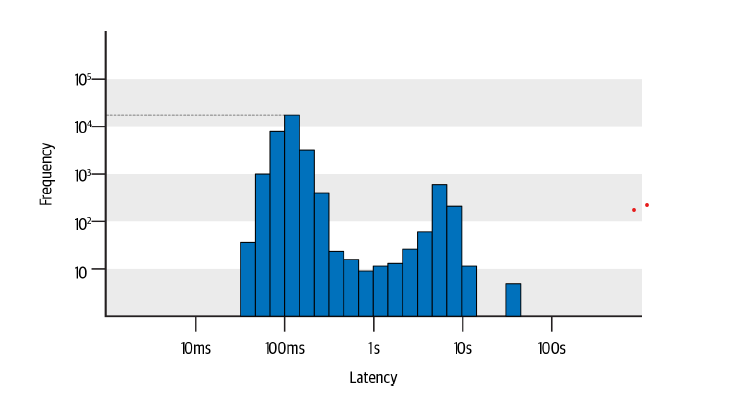
\includegraphics[width=1\textwidth]{resources/ch2/histogram-og.png}
	\caption{Contoh Histogram \citep{parker2020distributed}}
	\label{histogram}
\end{figure}

Ada beberapa teknik statistik yang dapat digunakan untuk mengetahui apakah dua buah sampel diambil dari sebuah distribusi yang sama. Salah satu teknik yang dapat digunakan adalah statistik Kolmogorov-Smirnov (K-S). Statistik K-S menghitung perbedaan dua buah distribusi sebagai sebuah bilangan skalar \citep{kolmogorov_1951}. Untuk mendapatkan distribusi tersebut, data yang berasal dari histogram akan terlebih dahulu diubah sebagai fungsi dengan fungsi distribusi kumulatif atau \textit{cumulative distribution function} (CDF). Ada dua perbedaan utama antara histogram dengan CDF. Pertama seperti namanya, CDF akan mengakumulasikan perhitungan, sehingga setiap titik pada CDF merupakan penjumlahan dari semua titik yang ada pada histogram di sebelah kiri. Kedua, sumbu y pada CDF dinormalisasi sehingga nilainya akan berkisar antara nol hingga satu. 

Gambar \ref{ks-example} menunjukkan dua buah CDF. Statistik K-S didapatkan dengan mencari jarak vertikal terjauh antara dua CDF seperti yang ditunjukkan oleh panah. Semakin besar jarak menunjukkan semakin mungkin bahwa dua buah CDF merupakan dua distribusi yang berbeda sehingga dapat menjadi indikasi bahwa terdapat perubahan pada kinerja. 
\begin{figure}[htb]
	\centering
	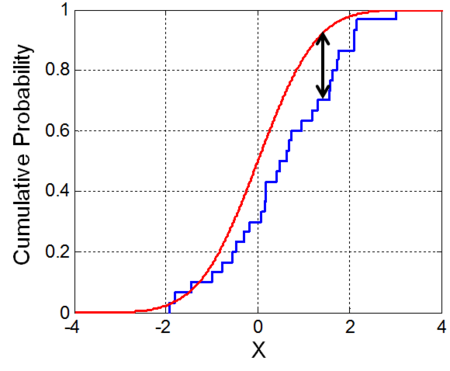
\includegraphics[width=0.6\textwidth]{resources/ch2/ks.png}
	\caption{CDF dari dua buah sampel, panah menunjukkan nilai statistik Kolmogorov-Smirnov \citep{wiki:ks-test}}
	\label{ks-example}
\end{figure}

\subsection{Analisis Agregasi dan Korelasi}
\label{approach-corr}

Langkah pertama dalam menggunakan pendekatan ini adalah dengan membagi hasil \textit{trace} menjadi dua kelompok sampel, kedua jenis sampel ini akan menjadi basis bagi semua perbandingan kedepannya. Dengan asumsi regresi sudah diketahui terjadi, sampel bagian pertama harus berasal dari regresi itu sendiri. Hal tersebut mudah didapatkan jika regresi sedang terjadi sekarang. Jika regresi juga terjadi pada sebagian besar dari \textit{request}, maka sampel dari \textit{request} tersebut juga dapat menjadi penting. 

Bagian sampel kedua harus berasal dari kinerja \textit{baseline}. Hal tersebut dapat berasal dari sekumpulan \textit{trace} sebelum regeresi terjadi, mungkin dari satu jam, satu hari, atau bahkan satu minggu sebelumnya; artinya adalah pertama kali sekali, sistem \textit{tracing} harus memiliki terlebih dahulu catatan mengenai kinerja \textit{baseline} dari aplikasi. Catatan kinerja \textit{baseline} dapat diperoleh dari siklus penggunaan aplikasi oleh pengguna. Penggunaan alat visualisasi seperti histogram dapat dilakukan untuk mengidentifikasi sampel mana yang dapat menjadi representasi \textit{baseline} dari aplikasi.

Setelah dimiliki dua kelompok sampel (misal sampel A dan B) dan juga sekelompok fitur, analisis dilakukan dengan melihat setiap fitur dan mengajukan pertanyaan "Apa kemungkinan fitur tersebut ada pada sampel A tetapi tidak ada di sampel B?". Pertanyaan tersebut akan menghasilkan "koefisien korelasi" bagi setiap fitur. Koefisien yang bernilai 1.0 berarti sebuah fitur ada pada setiap \textit{trace} pada sampel A dan tidak pernah ada pada sebuah \textit{trace} di sampel B, sementara koefisien -1.0 berarti sebuah fitur yang ada pada setiap \textit{trace} di sampel B dan tidak pernah ada pada \textit{trace} di sampel A. Sebuah koefisien 0.0 berarti fitur tersebut secara seimbang dapat ada pada kedua sampel. Semakin dekat hasil ke 1.0 atau -1.0 sebuah koefisien korelasi, semakin mungkin sebuah fitur dapat menjelaskan perbedaan antara kedua sampel.

Metrik-metrik seperti \textit{latency}, \textit{error}, \textit{tag}, dan metadata lainnya dapat menjadi fitur yang berharga dari \textit{trace} yang dapat digunakan untuk memahami perubahan apa yang telah terjadi. Salah satu keunggulan dari penggunaan \textit{distributed tracing} adalah dapat menempatkan perubahan kinerja dalam konteks apa yang terjadi pada alur keberjalanan aplikasi. Ketika menentukan atribut apa dari \textit{trace} mana saja yang akan digunakan sebagai bagian dari analisis korelasi, harus diingat bahwa atribut tersebut haruslah berasal dari setiap \textit{span} pada \textit{trace} yang ada, bukan hanya yang terkait dengan sebuah \textit{service} tertentu.

Sebagai contoh, andaikan telah terjadi peningkatan \textit{latency} pada \textit{service} yang ada dan sebagai tindakannya kita membandingkan sampel \textit{trace} yang terjadi pada lima menit terakhir dengan sampel \textit{trace} yang terjadi pada satu jam yang lalu. Tabel \ref{corr-tab-1} menunjukkan sampel kecil dari fitur yang dapat diidentifikasi oleh analisis ini.

\begin{small}
	\begin{longtable}{ | p{10cm} | p{2cm} | }
			\caption{Contoh analisis korelasi}
			\label{corr-tab-1}                                                           
			\\ \hline
			\centering\bfseries{Fitur} & \centering\bfseries{Koefisien Korelasi} \tabularnewline \hline
			\endfirsthead
			\textbf{service}: inventory, \textbf{service.version}: 1.14.2 & 0.65 \\ \hline
			\textbf{runinfo.host}: vm73 & 0.41 \\ \hline
			\textbf{service}: inventory, \textbf{service.version}: 1.14.1 &  $\num{-0.65}$ \\ \hline
		\end{longtable}
\end{small}

Tabel \ref{corr-tab-1} menunjukkan bahwa ada korelasi kuat antara versi baru dari \textit{service} "inventory" dengan hasil \textit{trace} terbaru. Terdapat orelasi yang kuat juga antara versi sebelumnya dengan hasil \textit{trace} yang berasal dari satu jam yang lalu. Hal tersebut memberikan cukup bukti untuk melakukan tindakan seperti melakukan \textit{rollback} ke versi sebelumnya untuk mengembalikan kinerja seperti semula.

Analisis agregasi juga dapat membantu untuk mengidentifikasi perubahan yang tidak terlalu nampak pada kinerja sebuah \textit{service}. Ketika membandingkan dua buah kumpulan \textit{trace}, kita dapat juga melihat kontribusi \textit{latency} yang terkait dengan \textit{tag}, operasi, dan \textit{service} dan juga melihat bagaimana kontribusi tersebut berubah sepanjang waktu.

Salah satu cara untuk melakukannya adalah dengan melihat bagaimana \textit{critical path} berubah diantara kumpulan \textit{trace} dari baseline dan juga kumpulan \textit{trace} yang terdampak regresi. \textit{Critical path} sendiri telah dibahas sebelumnya pada \ref{crit-path}. Dengan metode ini, \textit{critical path} akan dihitung pada setiap \textit{trace}. Rata-rata kontribusi metrik seperti \textit{latency} dari setiap \textit{service} dan operasinya akan ditentukan dari setiap kumpulan. Kemudian perbedaan rata-rata dari kontribusi metrik dari kumpulan \textit{baseline} dan regresi akan dihitung dan diurutkan sehingga dapat terlihat operasi atau \textit{service} mana yang sebenarnya menjadi akar dari penyebab regresi.

\begin{small}
	\begin{longtable}{ | p{5cm} | p{2cm} | p{2cm} | p{2cm} | }
		\caption{Kontribusi \textit{critical path} dalam \textit{trace} \textit{baseline} dan regresi}
		\label{corr-tab-2}                                                           
		\\ \hline
		\centering\bfseries{\textit{Service} / Operasi} & \centering\bfseries{\textit{Baseline}} & \centering\bfseries{Regresi} & \centering\bfseries{Perubahan} \tabularnewline \hline
		\endfirsthead
		inventory/write-cache & 63.1 ms & 368 ms & +305 ms \\ \hline
		inventory-db/update & 1.75 ms & 2.26 ms & +0.51 ms \\ \hline
		memcached/set & 4.94 ms & 4.71 ms & $\num{-0.23}$ ms \\ \hline
		inventory/update-inventory & 15.2 ms & 14.8 ms & $\num{-0.47}$ ms \\ \hline
		inventory/database-update & 32 ms & 30.6 ms & $\num{-1.4}$ ms \\ \hline
	\end{longtable}
\end{small}

Metode lain untuk memahami perubahan pada kinerja adalah untuk mempertimbangkan setiap \textit{tag} yang ditemukan pada semua kumpulan \textit{trace}. Untuk setiap \textit{tag}, semua \textit{span} pada setiap kumpulan yang memiliki sebuah \textit{tag} tertentu akan dienumerasi dan rata-rata durasi dari \textit{span} tersebut akan dihitung untuk setiap kumpulan \textit{trace}. Kemudian sama seperti metode sebelumnya akan diurutkan berdasarkan perubahan durasi dari \textit{baseline} dan regresi.

\begin{small}
	\begin{longtable}{ | p{5cm} | p{2cm} | p{2cm} | p{2cm} | }
		\caption{Rata-rata durasi \textit{span} dalam \textit{trace} \textit{baseline} dan regresi}
		\label{corr-tab-3}                                                           
		\\ \hline
		\centering\bfseries{\textit{Tag}} & \centering\bfseries{\textit{Baseline}} & \centering\bfseries{Regresi} & \centering\bfseries{Perubahan} \tabularnewline \hline
		\endfirsthead
		\textbf{item-type}: new & 114 ms & 1240 ms & +1130 ms \\ \hline
		\textbf{client.browser}: mozilla68 & 111 ms & 548 ms & +437 ms \\ \hline
		\textbf{db.instance}: cassandra.4 & 117 ms & 464 ms & +348 ms \\ \hline
		\textbf{runinfo.host}: vm123 & 115 ms & 453 ms & +337 ms \\ \hline
	\end{longtable}
\end{small}

Kedua metode, \textit{critical path} durasi total, dapat berperan penting dalam mencari akar masalah dari suatu permasalahan kinerja. Metode \textit{critical path} lebih baik digunakan untuk mengisolasi bagian kode mana yang mengonsumsi \textit{resource} sebagai bagian dari regresi, sementara durasi total dapat mendeteksi perubahan yang terjadi di luar dari sebuah kode atau modul yang sama. Terkadang perubahan hanya dihasilkan oleh sebuah kode atau konfigurasi baru yang di-\textit{deploy} tapi juga terkadang hasil dari interaksi antara kode lama dengan kode baru \citep{parker2020distributed}. 

\section{Penelitian Terkait}

%\subsection{Analisis Terotomasi dari \textit{Distributed Tracing}}
\subsection{Automated Analysis of Distributed Tracing}

\subsection{A Real-time Trace-level Root-cause Diagnosis System in Alibaba Datacenters}

\subsection{X-Trace}

\subsection{Dapper}

Dapper merupakan salah satu pionir teknologi \textit{distributed tracing} yang pertama kali dibuat oleh Google \citep{dapper-paper}. Dapper pertama kali dibuat untuk menyelesaikan permasalahan 

\subsection{Zipkin}

\subsection{Inkle}

